\documentclass[11pt]{article}
\usepackage[dvipsnames]{xcolor}
\usepackage{times}
\usepackage{amsmath,amsthm,amssymb,setspace,enumitem,epsfig,titlesec,verbatim,array,eurosym,multirow}
\usepackage[sort&compress,numbers]{natbib}
\usepackage[footnotesize,bf]{caption}
\usepackage[margin=2.5cm, includefoot, footskip=30pt]{geometry}
\usepackage{standalone}
\usepackage{tikz}
\usepackage{subcaption}
\usepackage{hyperref}
\usepackage{tabularx}
\usepackage{booktabs}
\usepackage{blkarray}
\usepackage[ruled,vlined]{algorithm2e}
\smallskip % Erlaubt kleine Abstaende zwischen Paragraphen, falls es dem Seitenlayout hilft
\renewcommand{\baselinestretch}{1.15}
\usepackage{tikz}
\usetikzlibrary{arrows}
\usepackage{minitoc}
\usepackage{graphicx}
\usepackage{hyperref}
\usepackage{subcaption}
\usepackage{multirow}
\usepackage{multicol}
\usepackage{standalone}

\newcommand{\nikoleta}[1]{\textcolor{orange}{\textbf{NG}: #1}}
\newcommand{\christian}[1]{\textcolor{blue}{\textbf{CH}: #1}}

\newtheoremstyle{plainCl1}% name
{12pt}%      Space above, empty = 'usual value'
{12pt}%      Space below
{\it}% 	   Body font
{}%         Indent amount (empty = no indent, \parindent = para indent)
{\bfseries}% Thm head font
{}%        Punctuation after thm head
{\newline}% Space after thm head: \newline = linebreak
{}%         Thm head spec

\theoremstyle{plainCl1}
\newtheorem{theorem}{Theorem}
\newtheorem{lemma}{Lemma}
\newtheorem{corollary}{Corollary}
\newtheorem{proposition}{Proposition}


\newtheoremstyle{plainCl2}% name
{12pt}%      Space above, empty = 'usual value'
{12pt}%      Space below
{}% 	   Body font
{}%         Indent amount (empty = no indent, \parindent = para indent)
{\bfseries}% Thm head font
{}%        Punctuation after thm head
{\newline}% Space after thm head: \newline = linebreak
{}%         Thm head spec

\theoremstyle{plainCl2}
\newtheorem*{definition}{Definition}



\def\wsls{\texttt{WSLS}}
\def\tft{\texttt{TFT}}
\def\gtft{\texttt{GTFT}}
\def\allc{\texttt{ALLC}}
\def\alld{\texttt{ALLD}}
\def\alt{\texttt{Alternator}}



\titleformat{\section}{\sffamily \fontsize{12}{15}\bfseries}{\thesection}{0.4em}{}
\titleformat{\subsection}{\sffamily\fontsize{11}{15}\bfseries}{\thesubsection}{0.4em}{}
\renewcommand{\thefigure}{S\arabic{figure}}




\title{~\\[-1.5cm]{\sffamily \Large Revision notes}\\[-0.3cm]}

\date{\empty}

\begin{document}
%% DEFECTING STRATEGIES: Donation Game %%

\section{Reactive defecting Nash strategies in the donation game}\label{section:defecting_donation_game}

In the previous section, we have characterized the reactive partner strategies
for a special case of the donation game and the general prisoner's dilemma. In
the following, we apply the same methods based on Section~\ref{Sec:Algorithm} to
analyze defecting Nash equilibria. For the case of reactive-1 strategies, we
obtain the following characterization.

%% DEFECTING STRATEGIES: Reactive-1 Donation Game %%

\begin{theorem}[Reactive-1 defecting Nash strategies in the donation game]
\label{theorem:reactive_one_defecting_strategies}
A reactive-1 strategy $\mathbf{p}$ is a defecting Nash strategy if and only if
its entries satisfy the conditions

\begin{equation}
  \begin{array}{rcl}
    p_{C} \le  \frac{c}{b} \qquad \text{ and } \qquad  p_{D} \!=\! 0.
\end{array}
\end{equation}
\end{theorem}


%% DEFECTING STRATEGIES: Reactive-2 Donation Game %%

\begin{theorem}[Reactive-2 defecting Nash strategies in the donation game]
\label{theorem:reactive_two_defecting_strategies}
A reactive-2 strategy $\mathbf{p}$ is a defecting Nash strategy if and only if
its entries satisfy the conditions

\begin{equation}\label{eq:defecting_conditions_two}
  p_{CC} \le \frac{c}{b}, \qquad \displaystyle \frac{p_{CD} \!+\! p_{DC}}{2} \le \frac{c}{2b}, \qquad p_{DD} = 0.
\end{equation}
\end{theorem}

%% DEFECTING STRATEGIES: Reactive-3 Donation Game %%

\begin{theorem}[Reactive-3 defecting Nash strategies in the donation game]
\label{theorem:reactive_three_defecting_strategies}
A reactive-3 strategy $\mathbf{p}$ is a defecting Nash strategy if and only if
its entries satisfy the conditions

\begin{align}\label{eq:defecting_conditions_three}
  \begin{split}
  p_{CCC} & \le \frac{c}{b} \\
  \frac{p_{CDC} + p_{DCD}}{2} & \leq \frac{1}{2} \cdot \frac{c}{b} \\
  \frac{p_{CCD} + p_{CDC} + p_{DCC}}{3} & \leq \frac{2}{3} \cdot \frac{c}{b} \\
  \frac{p_{CDD} + p_{DCD} + p_{DDC}}{3} & \leq \frac{1}{3} \cdot \frac{c}{b} \\
  \frac{p_{CCD} + p_{CDD} + p_{DCC} + p_{DDC}}{4}  & \leq \frac{1}{2} \cdot \frac{c}{b}  \\
  p_{DDD} & = 0.
  \end{split}
\end{align}

\end{theorem}

We repeat the same analysis for reactive counting strategies. We obtain the
following results.

%% DEFECTING STRATEGIES: Reactive-2 Counting Donation Game %%

\begin{theorem}[Reactive-2 defecting Nash counting strategies in the donation game]
\label{theorem:reactive_two_defecting_counting_strategies}
A reactive-2 counting strategy $\mathbf{r}$ is a defecting Nash strategy if and only if
its entries satisfy the conditions

\begin{equation}\label{eq:defecting_conditions_two_counting}
  r_{2} \le \frac{c}{b}, \qquad \displaystyle r_{1} \le \frac{1}{2} \cdot \frac{c}{b}, \qquad r_{0} = 0.
\end{equation}
\end{theorem}

%% DEFECTING STRATEGIES: Reactive-3 Counting Donation Game %%

\begin{theorem}[Reactive-3 defecting Nash counting strategies in the donation game]
\label{theorem:reactive_three_defecting_counting_strategies}
A reactive-3 counting strategy $\mathbf{r}$ is a defecting Nash strategy if and only if
its entries satisfy the conditions

\begin{equation}\label{eq:defecting_conditions_three_counting}
  r_{3} \le \frac{c}{b}, \qquad r_{2} \leq\frac{2}{3} \cdot \frac{c}{b}, \qquad
  r_{1} \leq\frac{1}{3} \cdot \frac{c}{b}, \qquad
  r_{0} = 0.
\end{equation}

\end{theorem}


\noindent
We can observe that for each value of \(n\), the left-hand side of the
conditions for cooperative and defective Nash are the same. Moreover, it is
clear that the right-hand side of the defective Nash conditions is always
strictly smaller than those of the cooperative Nash conditions. This means that
within the space of feasible strategies, the volume of partner strategies is
always larger than the volume of defective Nash strategies. We verified these
analytical results numerically as well.

We selected random strategies from the feasible space of strategies and created
two copies of each strategy. For one copy, we set the probability of cooperating
after full cooperation of the co-player to 1 (for example, for reactive-1, \(p_{C} = 1\)). 
For the second copy, we set the probability of cooperating after
full defections of the co-player to 0 (for example, for reactive-2, \(p_{DD} =
0\)). We then checked if either copy is Nash: cooperative for the first and
defective for the second. We repeated this process for \(10^4\) randomly
selected strategies and plotted the relative volumes of cooperative and
defective Nash equilibria (Figure~\ref{fig:reactive_volume}). We also verified
that this holds true for different values of cost.

\begin{figure}[t]
  \centering
  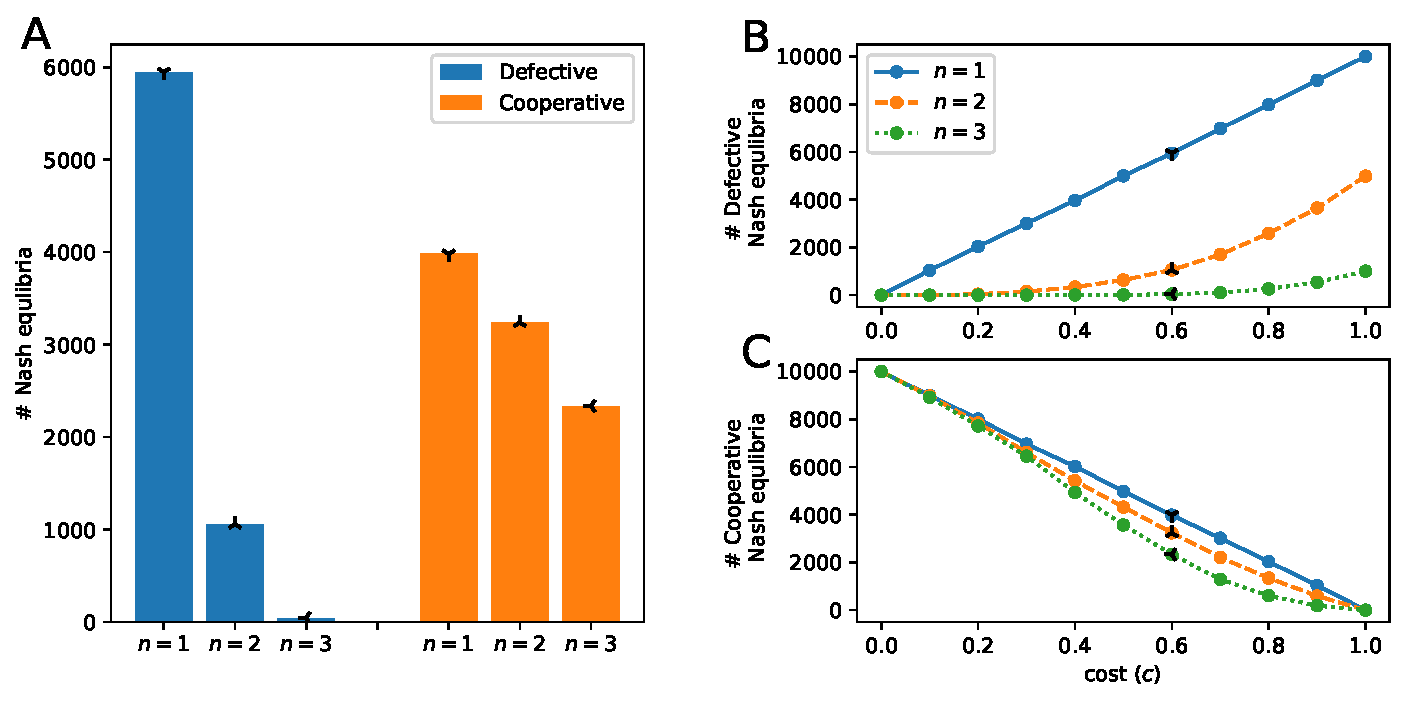
\includegraphics[width=\textwidth]{../../figures/siFig1.pdf}
  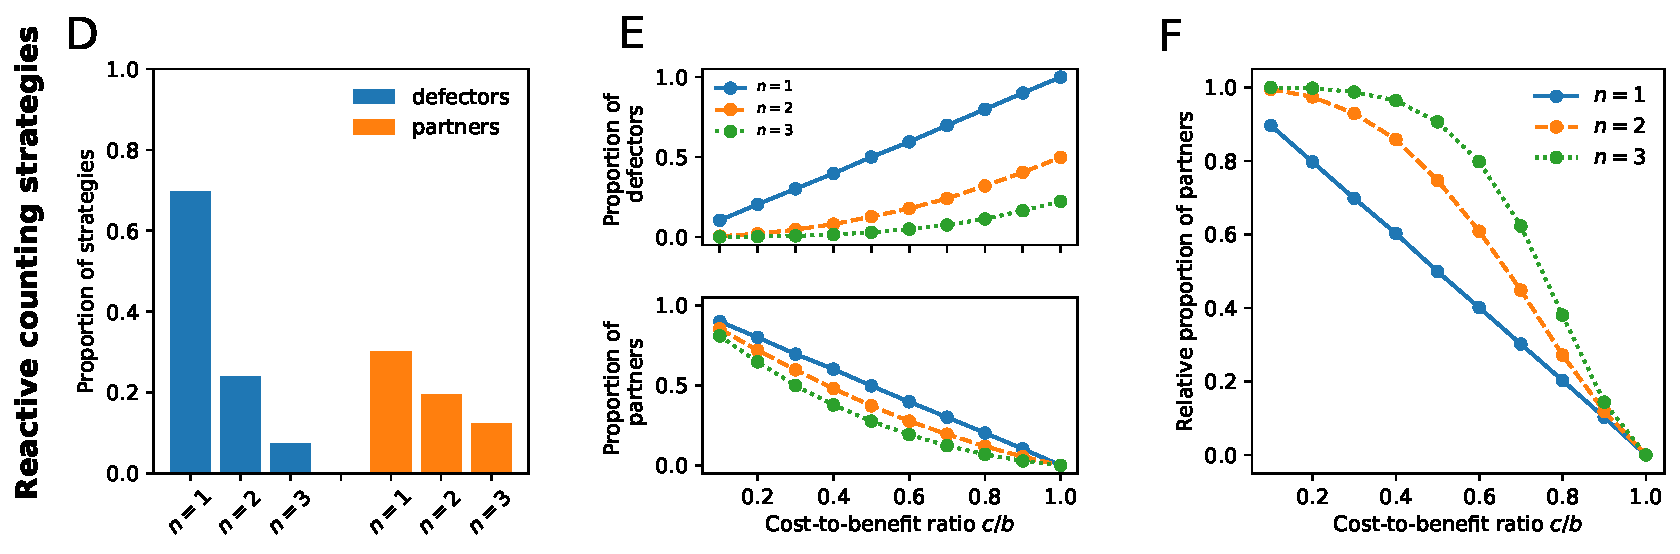
\includegraphics[width=\textwidth]{../../figures/siFig1Counting.pdf}
  \caption{
  \textbf{Volume of cooperative and defective Nash.}
We draw \(10^4\) random
strategies from the feasible space of strategies and create two copies of each
strategy. For one copy, we set the probability of cooperating after full
cooperation of the co-player to 1. For the second copy, we set the probability
of cooperating after full defections of the co-player to 0. We then checked if
either copy is Nash: cooperative for the first and defective for the second. We
set the benefit of cooperation to \(b = 1\). 
{\bf A} We plot the results for a given value of cost, \(c = 0.5\).
{\bf B} The number of defective Nash strategies as a function of cost.
{\bf C} The number of cooperative Nash strategies as a function of cost.
}\label{fig:reactive_volume}
\end{figure}


%%%%%%%%%%%%%%%%%%%%%%%%%%%%%
%% Evolutionary Simulations  %%
%%%%%%%%%%%%%%%%%%%%%%%%%%%

\section{Evolutionary Simulations}

We perform the evolutionary analysis of Figure 3 of the main text. We simulate
the evolutionary process twenty times this time,
Figure~\ref{fig:evolutionary_results}. Now, one question that arises is how many
of these strategies are actually partner strategies? And for the partner
strategies, do we see all of them represented? \\

\begin{figure}[tbhp]
    \centering
    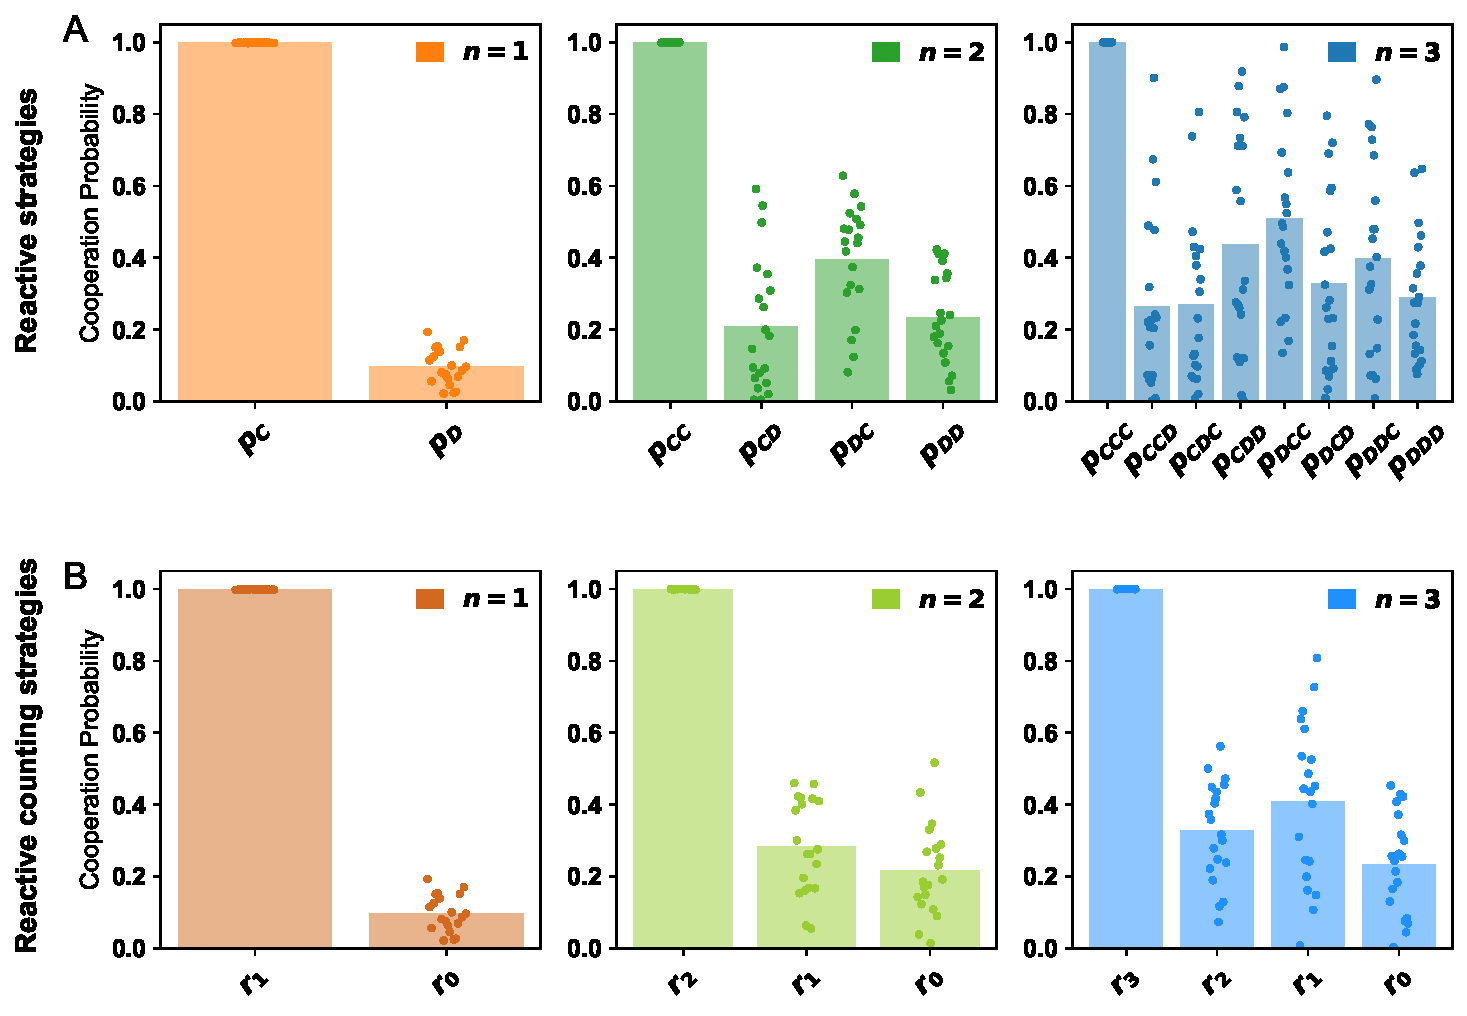
\includegraphics[width=\textwidth]{../../figures/siFig3AbundantStrategies.pdf}
    \caption{\textbf{Evolutionary dynamics of reactive-$n$ strategies.}
    To explore the evolutionary dynamics among reactive-$n$ strategies, we run simulations based on the
    method of Imhof and Nowak. 
    This method assumes rare mutations. 
    Every time a mutant strategy appears, it goes extinct or fixes before the arrival of the next mutant strategy. 
    We run twenty independent simulations for reactive-$n$ strategies.
    For each simulation, we record the most abundant strategy (the strategy that resisted most mutants). 
    The respective average cooperation probabilities are in line with the conditions for partner strategies. 
    Simulations are based on a donation game with \(b\!=\!1\),  \(c\!=\!0.5\), a selection strength $\beta\!=\!1$
    and a population size $N\!=\!100$, unless noted otherwise. For $n$ equal to 1 and 2, simulations are run for \(T\!=\! 10 ^ 7\) time steps. For $n\!=\!3$ we use \(T\!=\! 2 \!\cdot\!10 ^ 7\) time steps.
    }\label{fig:evolutionary_results}
\end{figure}


\begin{figure}[tbhp]
  \centering
  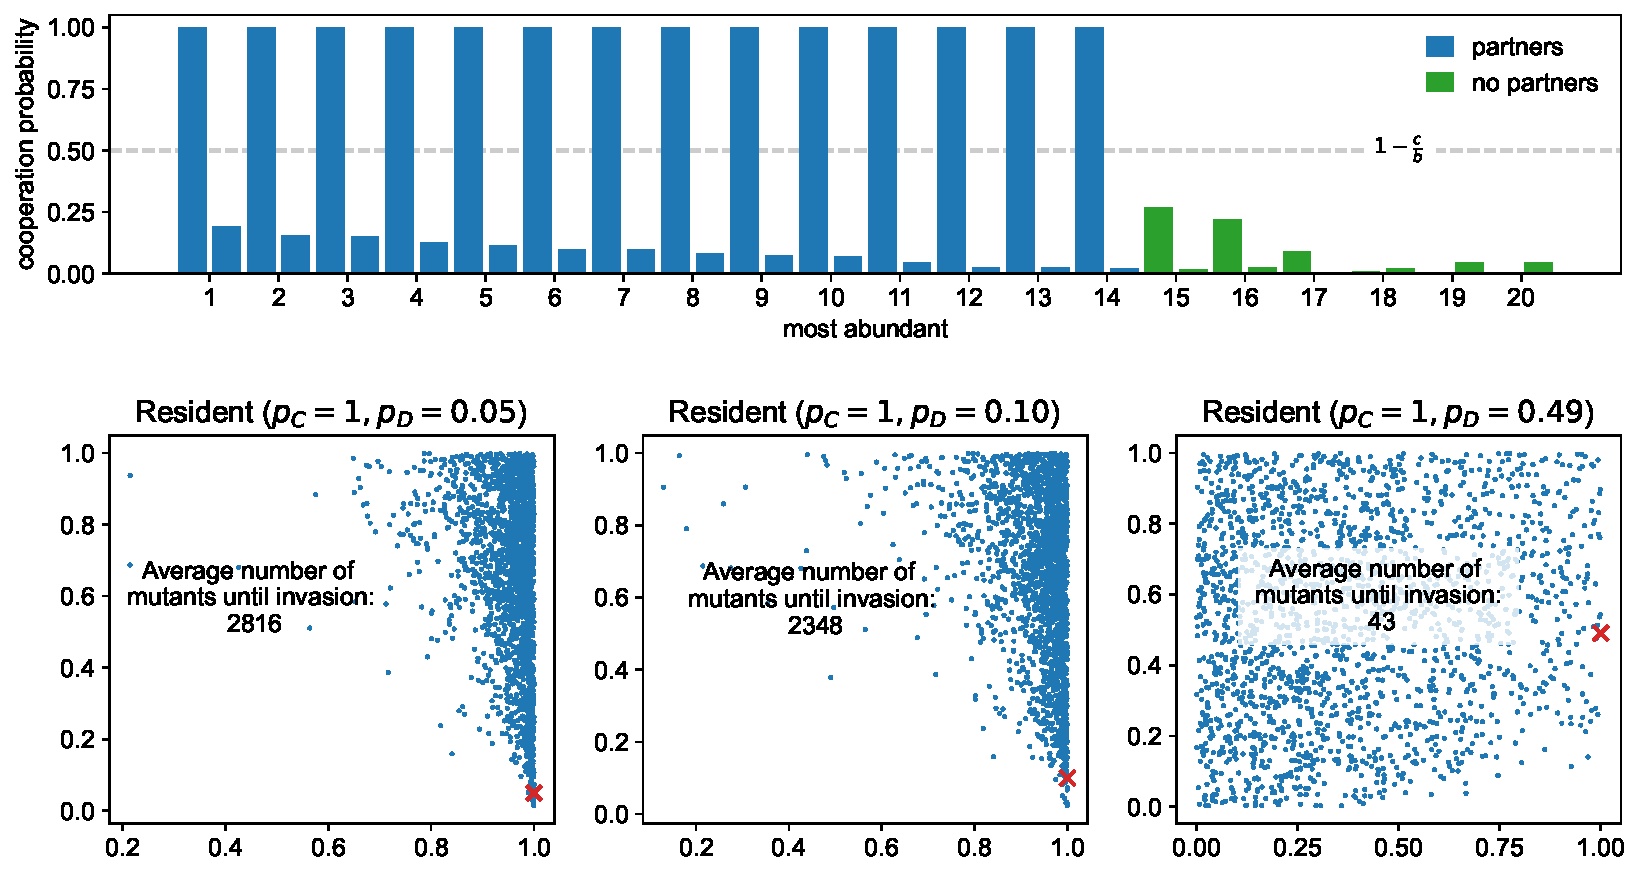
\includegraphics[width=\textwidth]{../../figures/siFigInvasionR1.pdf}
  \caption{\textbf{Invasion analysis for reactive-1.}
  }
\end{figure}

\begin{figure}[tbhp]
  \centering
  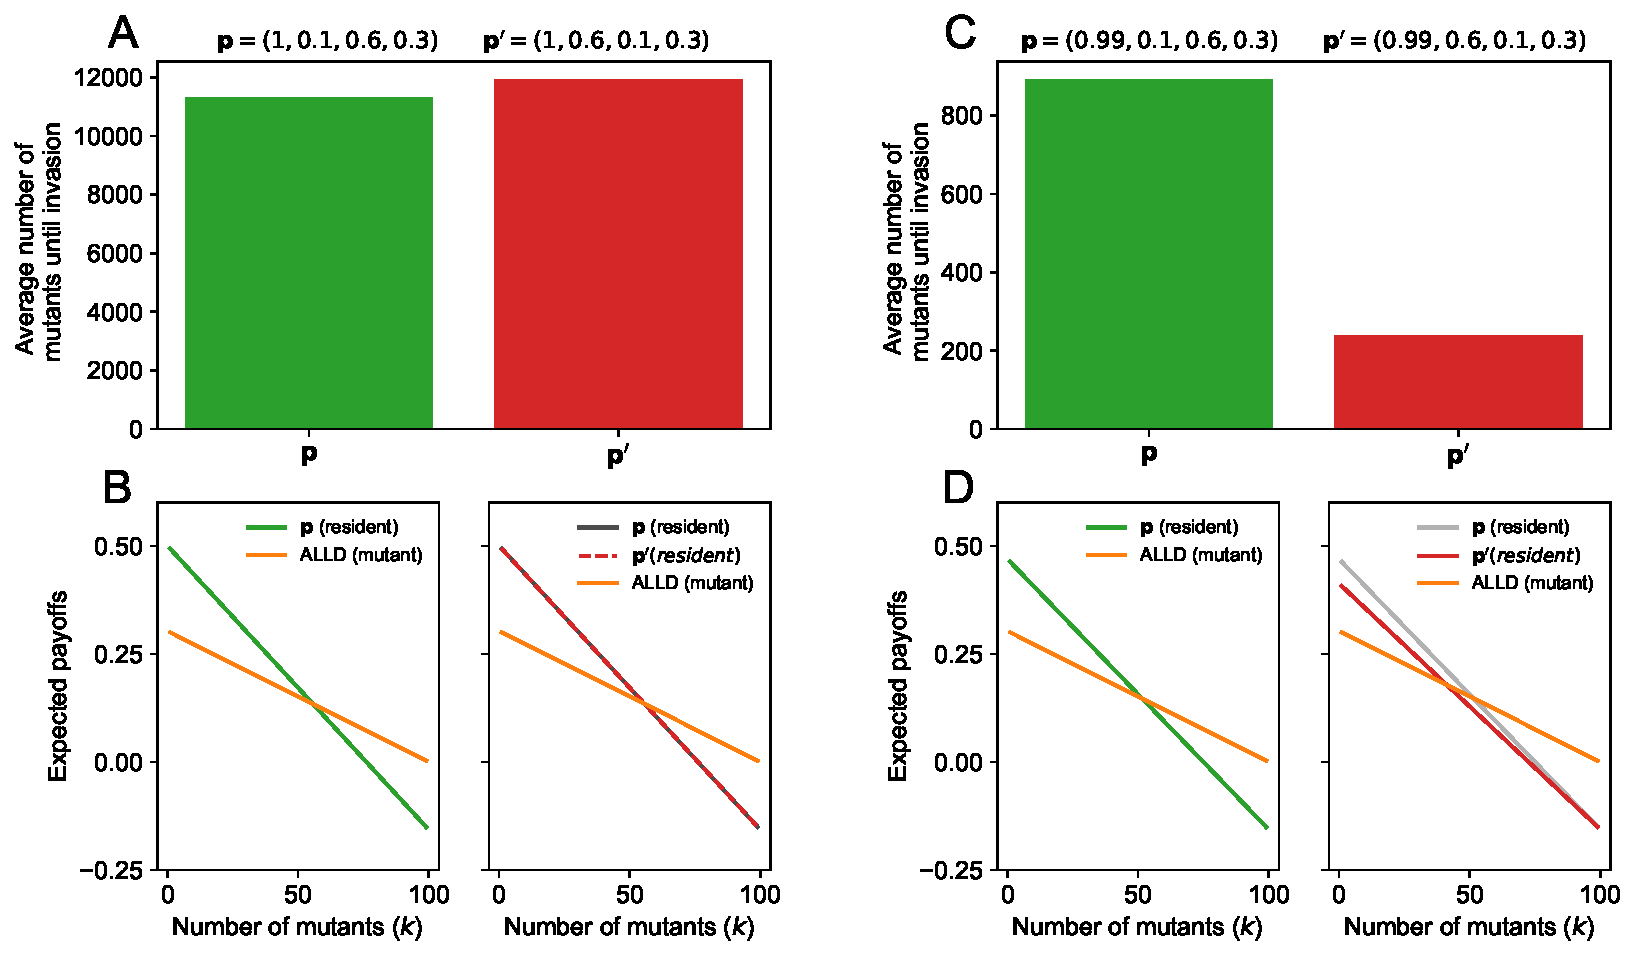
\includegraphics[width=\textwidth]{../../figures/siFigInvasionR2.pdf}
  \caption{\textbf{Invasion analysis for reactive-1.}
  }
\end{figure}



\noindent
\textbf{Reactive-1 strategies.} In the case of reactive-1, all the most abundant
strategies are partner strategies. However, from Eq. and for a given value of c,
the probability of defecting is... However, we observe only a lower value of \(
p_{dd} \), thus only some partner strategies are residents. This result is not
explained by the theory. To better understand this result, we need to do an
invasion analysis. For the invasion analysis, we consider a given resident
strategy, and we sample \( 10^3 \) random strategies to estimate if this mutant
will invade the resident. We record the number of mutants that took over. We
repeat this \( 10^3 \) times. The results are shown in Fig. X, and what we
observe is that a lower value of \( p_{dd} \) results in a more robust strategy
to invasion, as only cooperative strategies on the GTFT can take over, in
comparison with panel B where defective strategies are more likely to invade.

\noindent
\textbf{Reactive-12strategies.} In the case of reactive-2, we observe that almost all
strategies are partner strategies. However, what seems to be the case is that \(
p_{dc} \) is higher on average than \( p_{cd} \). In order to understand this,
we again run an invasion analysis. This time we also consider two values of \(
p_{dd} \). The results are shown in Fig. Y. \\


%%%%%%%%%%%%
%% Errors  %%
%%%%%%%%%%%%

\section{Errors}

So far, we have considered the case where there cannot be a mistake in the
actions taken by a player; the actions of the players are realized without
error. Here, we discuss what happens in the case where such an error is
possible. More specifically, we consider that \(\epsilon\) is the probability
that a player makes a mistake in the action taken.

\begin{figure}[t]
    \centering
    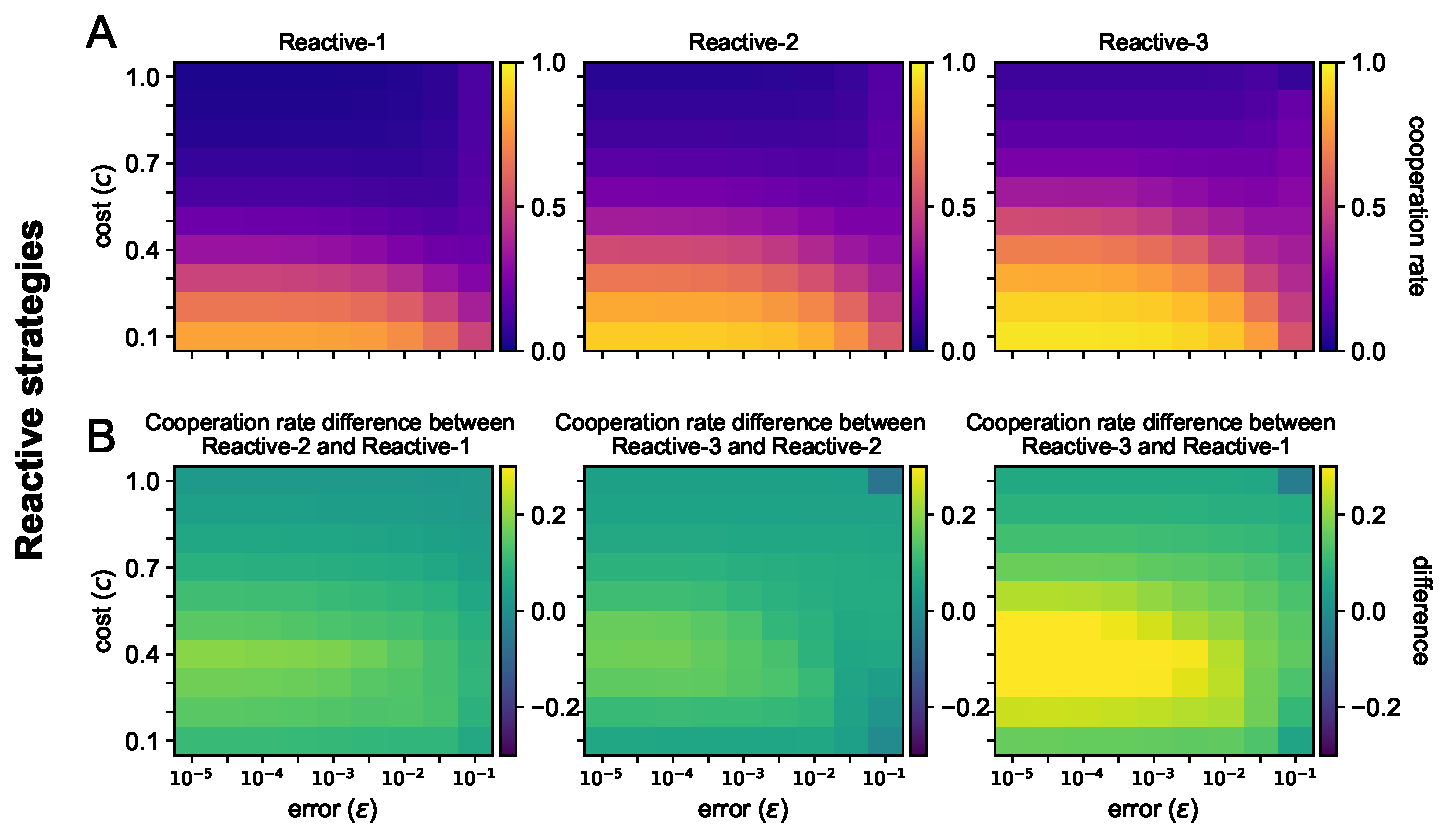
\includegraphics[width=\textwidth]{../../figures/siFig2Errors.pdf}
    \caption{
    \textbf{Cooperating rates with implementation errors.}
We simulate the evolutionary process, this time allowing for implementation
errors. Specifically, we consider a probability \(\epsilon\) that a player makes a mistake
in the action taken. We calculate the average cooperation rate for different
values of \(\epsilon\) and \(c\).
{\bf A} We plot the average cooperation rate for the different parameters when
individuals use reactive-1, reactive-2, and reactive-3 strategies, respectively.
{\bf B} We plot the differences between the cooperation rates when individuals use
different memory size strategies. From left to right, we show the differences
between reactive-1 and reactive-2, reactive-2 and reactive-3, and reactive-1 and
reactive-3 strategies.
    }\label{fig:errors}
\end{figure}

\end{document}